\section{Overall Accuracy}
The 
    \begin{figure}[!htb]
        \begin{center}
          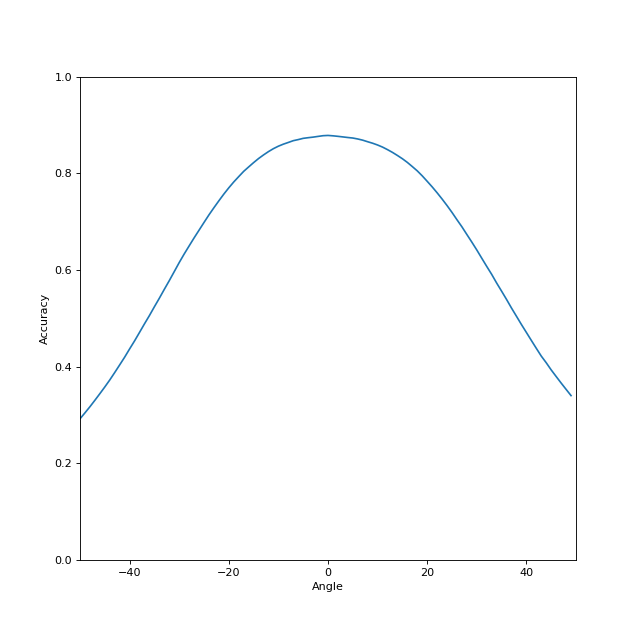
\includegraphics[scale=0.6]{chapters/results/CNN/Rotate/acc.png}
          \caption{Overall accuracy for metamorphic relation rotation.}
          \label{fig:Rotate 1}
        \end{center}
    \end{figure}
    
\clearpage
    \begin{figure}[!htb]
    \centering
      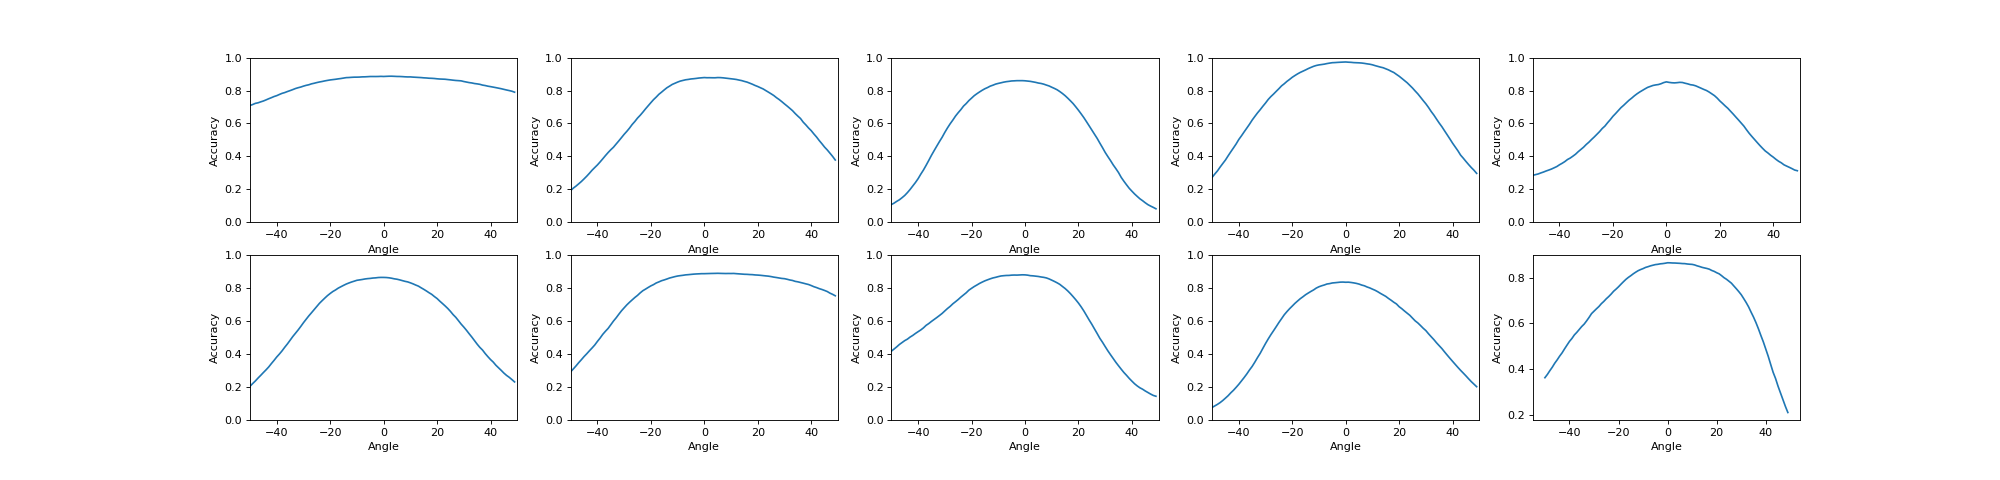
\includegraphics[width=\linewidth]{chapters/results/CNN/Rotate/accAll.png}
      \caption{Accuracy of each digit.}
      \label{fig: Shading}
    \end{figure}
        
\clearpage
\begin{figure}[htb!]
    \centering
    \begin{subfigure}[b]{\textwidth}
        \centering
        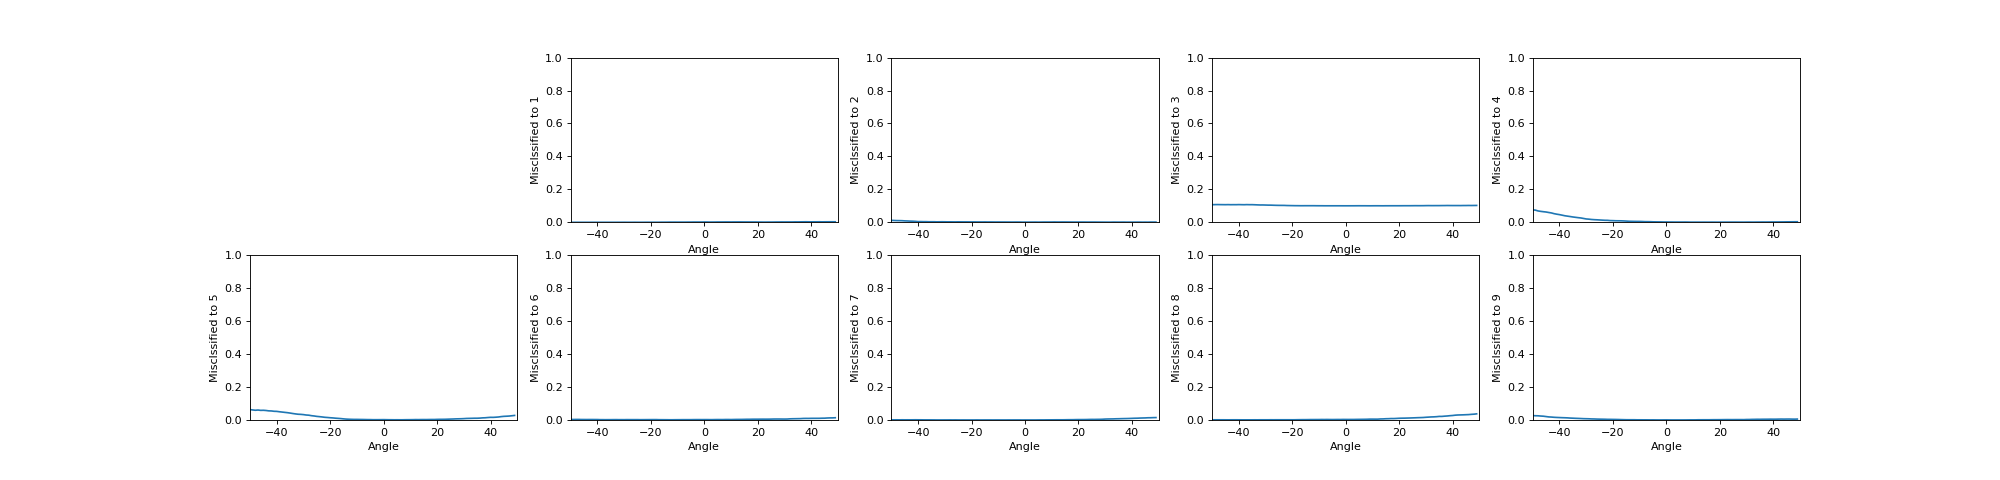
\includegraphics[width=\textwidth]{chapters/results/CNN/Rotate/acc1.png}
        \caption{Misclassification of Digit 0}
        \label{fig:Rotate-misclass0}
    \end{subfigure}
    \begin{subfigure}[b]{\textwidth}
        \centering
        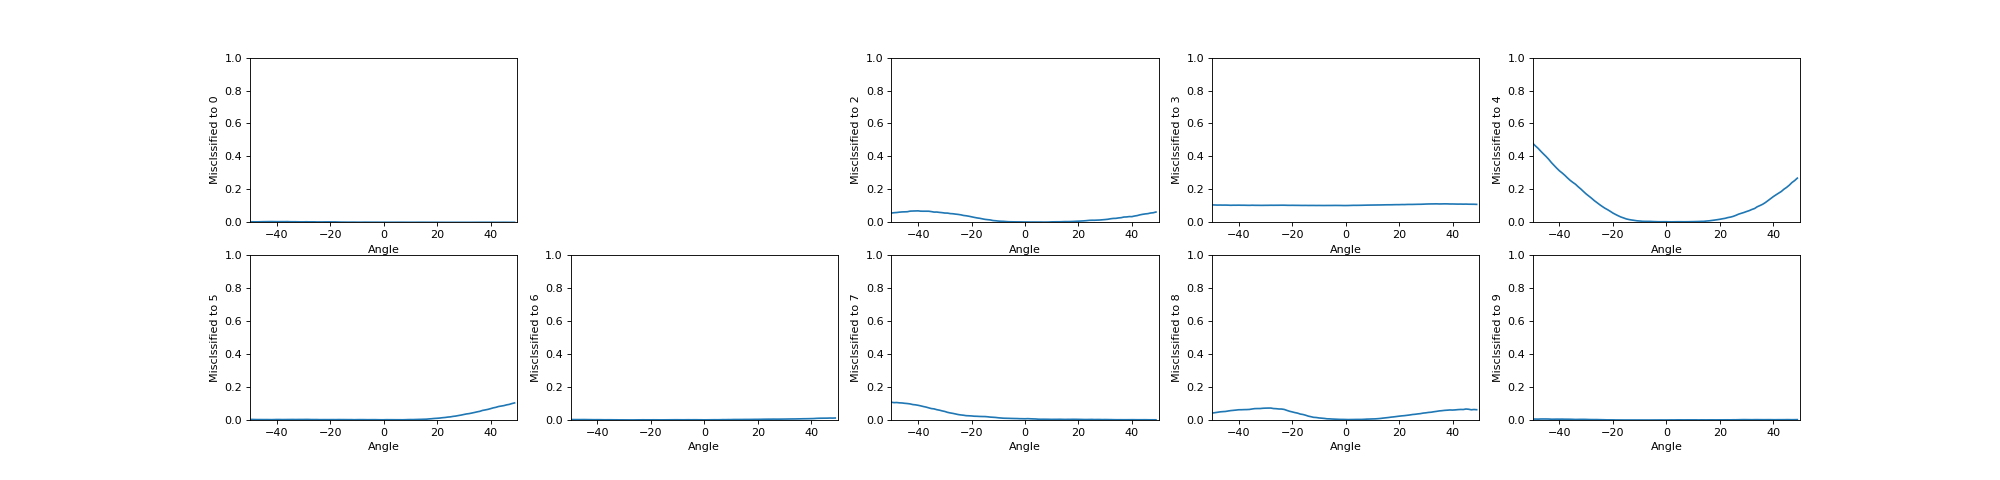
\includegraphics[width=\textwidth]{chapters/results/CNN/Rotate/acc2.png}
        \caption{Misclassification of Digit 1}
        \label{fig:Rotate-misclass0}
    \end{subfigure}
    \begin{subfigure}[b]{\textwidth}
        \centering
        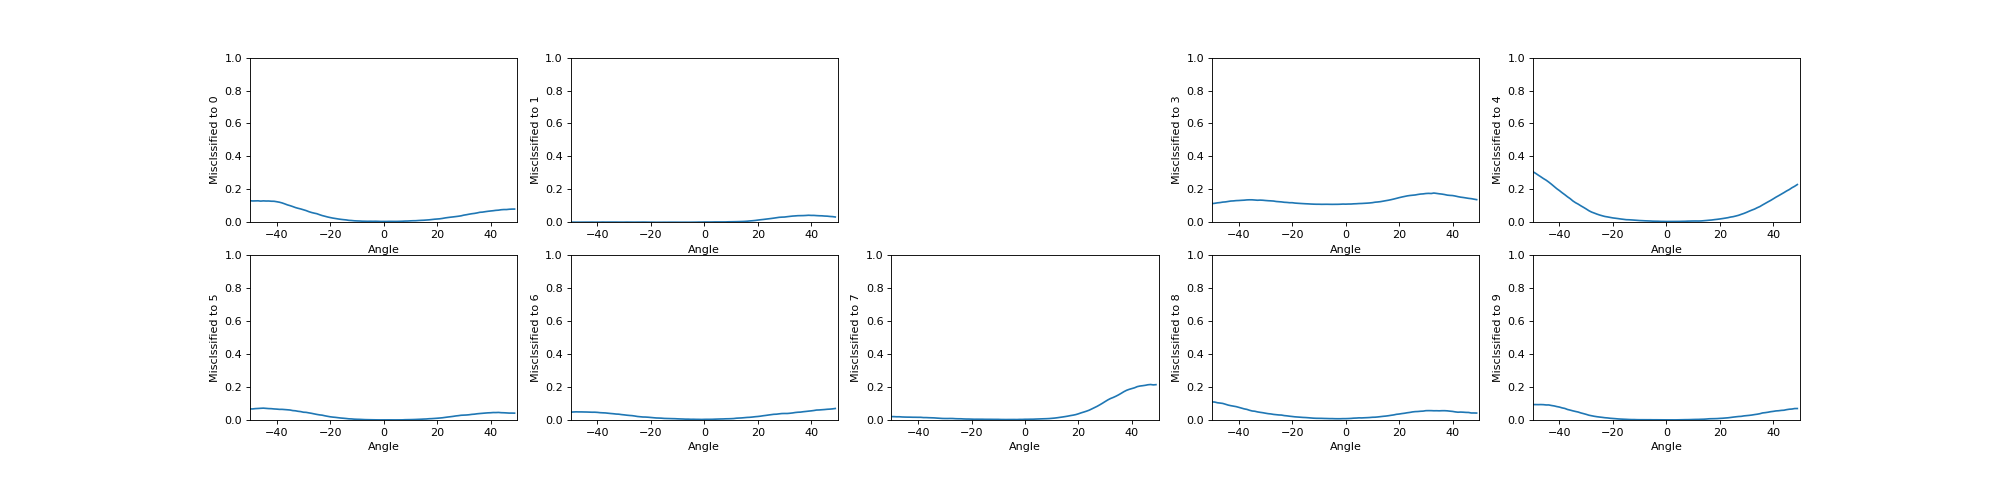
\includegraphics[width=\textwidth]{chapters/results/CNN/Rotate/acc3.png}
        \caption{Misclassification of Digit 2}
        \label{fig:Rotate-misclass0}
    \end{subfigure}
    \begin{subfigure}[b]{\textwidth}
        \centering
        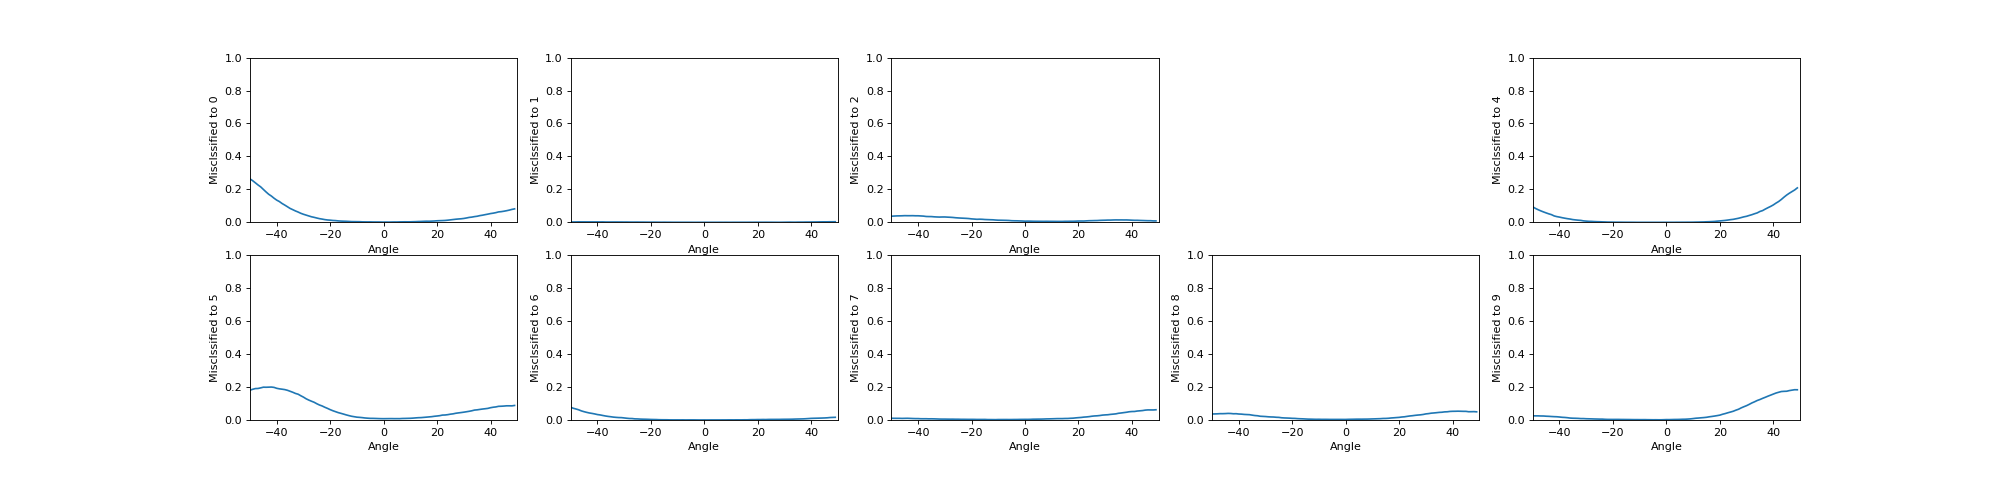
\includegraphics[width=\textwidth]{chapters/results/CNN/Rotate/acc4.png}
        \caption{Misclassification of Digit 3}
        \label{fig:Rotate-misclass0}
    \end{subfigure}
    \begin{subfigure}[b]{ \textwidth}
        \centering
        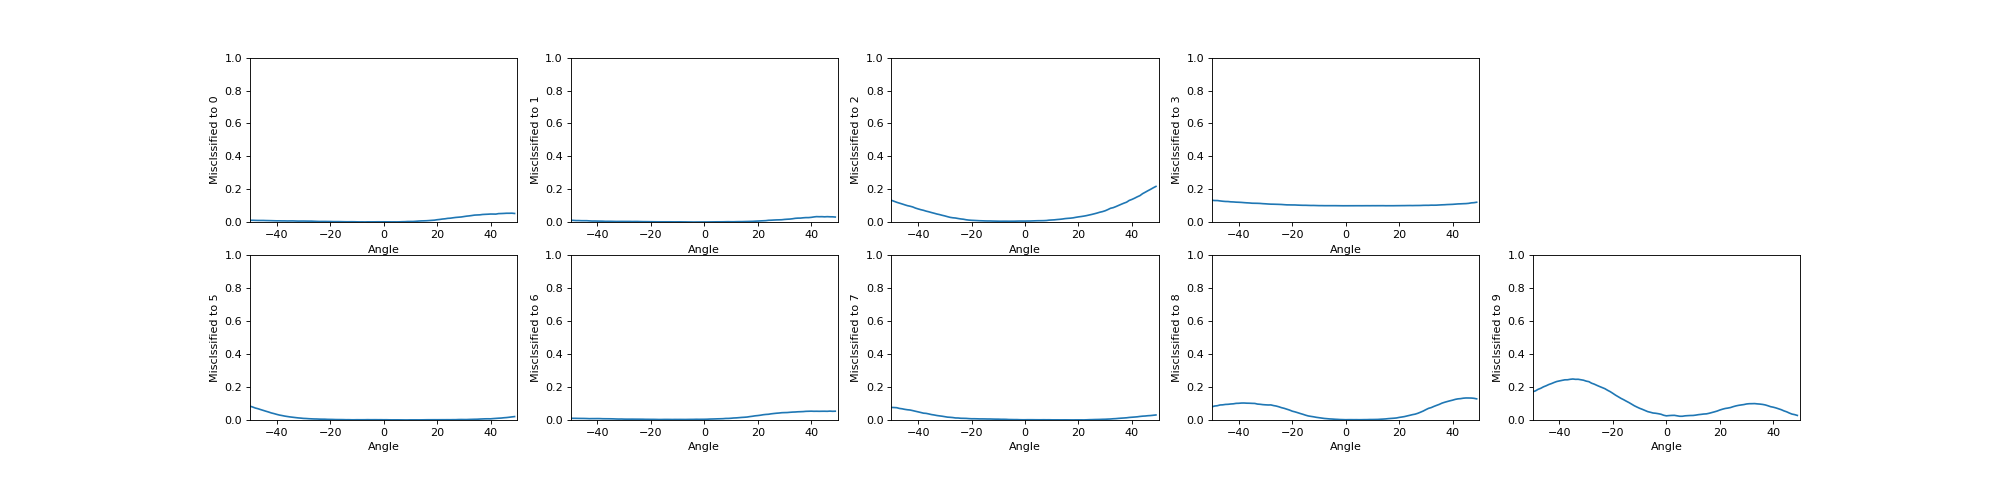
\includegraphics[width=\textwidth]{chapters/results/CNN/Rotate/acc5.png}
        \caption{Misclassification of Digit 4}
        \label{fig:Rotate-misclass1}
    \end{subfigure}
    \caption{Misclassification.}
    \label{fig:Rotate-misclassifications}
\end{figure}

\clearpage
\begin{figure}[htb!]
    \centering
    \begin{subfigure}[b]{\textwidth}
        \centering
        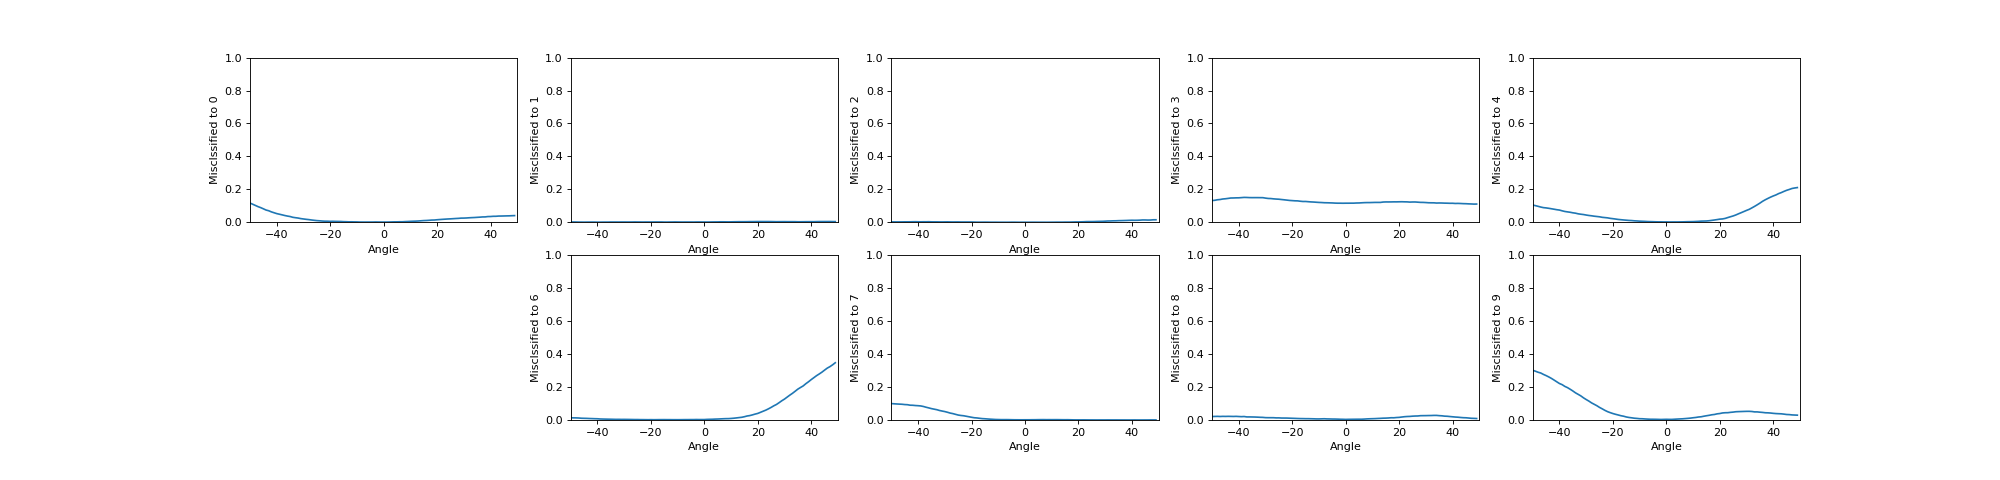
\includegraphics[width=\textwidth]{chapters/results/CNN/Rotate/acc6.png}
        \caption{Misclassification of Digit 5}
        \label{fig:Rotate-misclass0}
    \end{subfigure}
    \begin{subfigure}[b]{\textwidth}
        \centering
        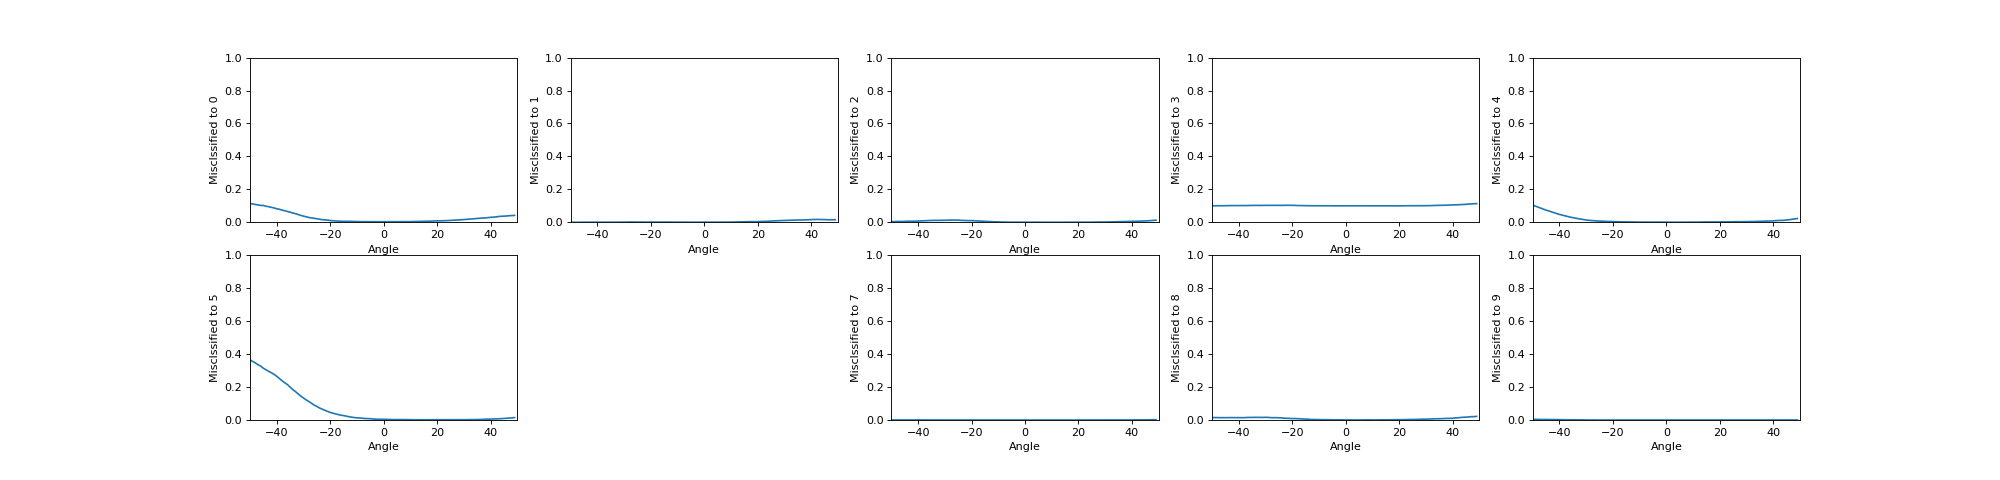
\includegraphics[width=\textwidth]{chapters/results/CNN/Rotate/acc7.png}
        \caption{Misclassification of Digit 6}
        \label{fig:Rotate-misclass0}
    \end{subfigure}
    \begin{subfigure}[b]{\textwidth}
        \centering
        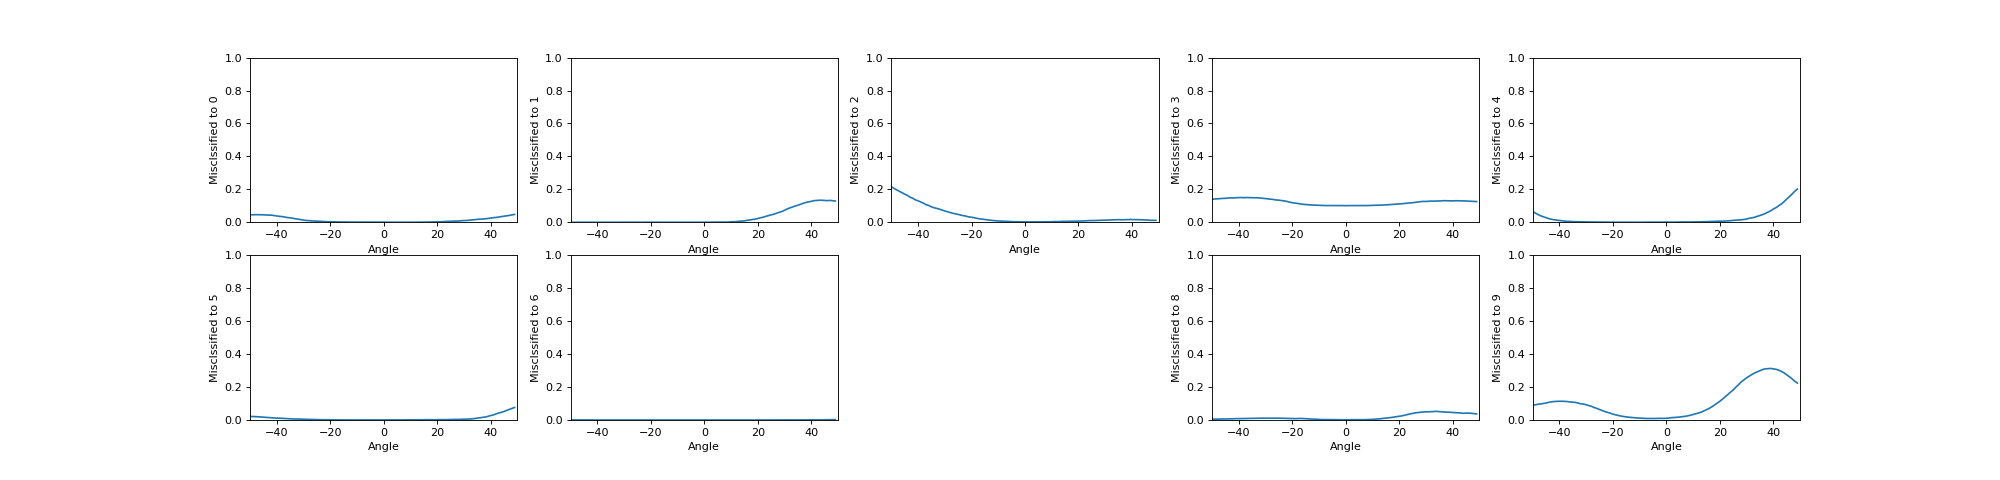
\includegraphics[width=\textwidth]{chapters/results/CNN/Rotate/acc8.png}
        \caption{Misclassification of Digit 7}
        \label{fig:Rotate-misclass0}
    \end{subfigure}
    \begin{subfigure}[b]{\textwidth}
        \centering
        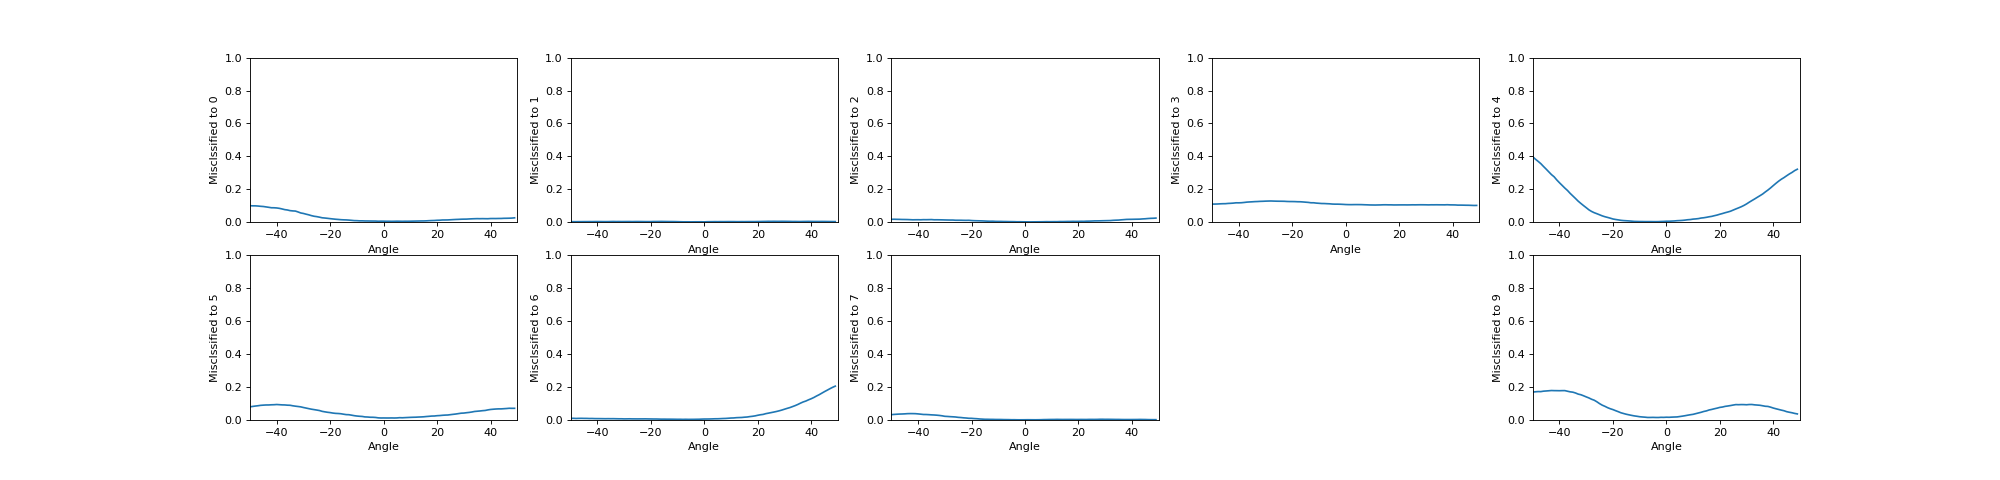
\includegraphics[width=\textwidth]{chapters/results/CNN/Rotate/acc9.png}
        \caption{Misclassification of Digit 8}
        \label{fig:Rotate-misclass0}
    \end{subfigure}
    \begin{subfigure}[b]{ \textwidth}
        \centering
        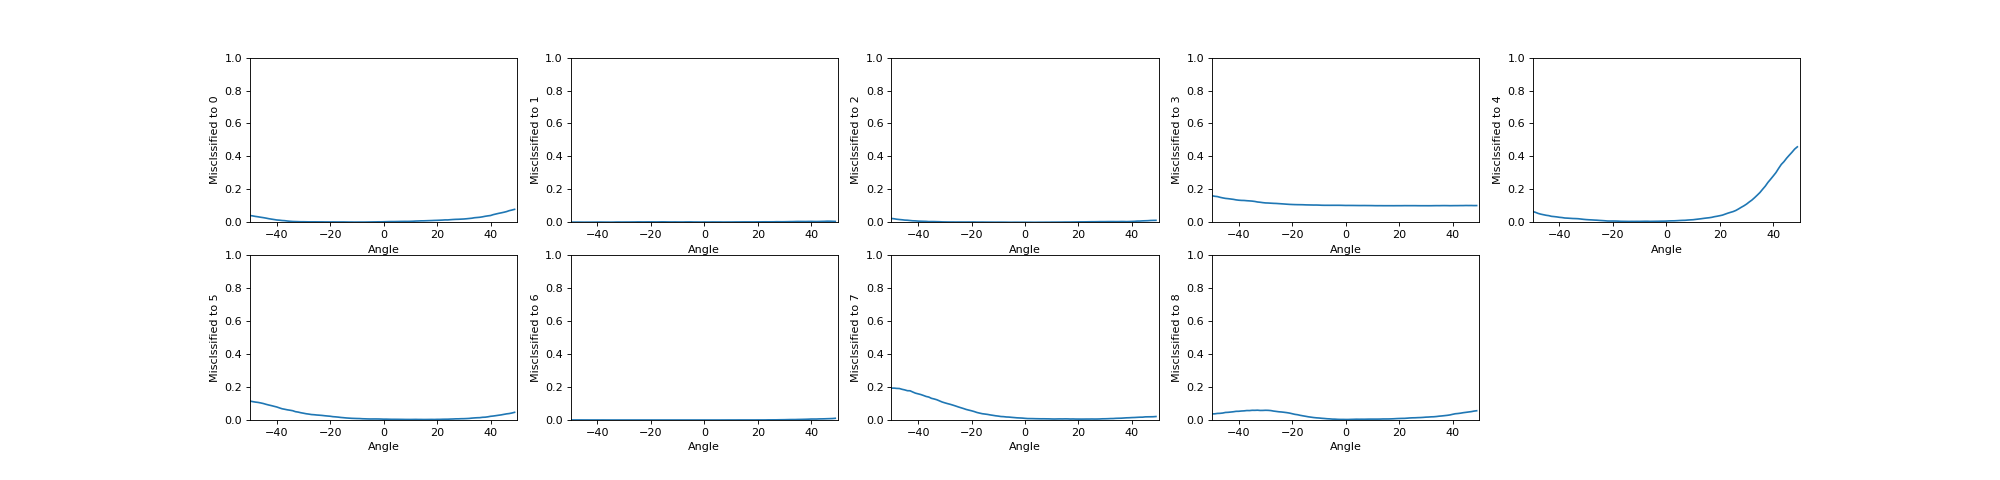
\includegraphics[width=\textwidth]{chapters/results/CNN/Rotate/acc10.png}
        \caption{Misclassification of Digit 9}
        \label{fig:Rotate-misclass1}
    \end{subfigure}
    \caption{Caption for all subfigures.}
    \label{fig:Rotate-misclassifications}
\end{figure}
        
\clearpage
